Negativ-parallaxe Bildausschnitte können wie in Kapitel \ref{chp:wahrnehmungskonflikte_und_loesungsansaetze} beschrieben Wahrnehmungskonflikte hervorrufen. In diesem  Kapitel wird die im Rahmen dieser Arbeit entstandene \emph{See-Through} Technik basierend auf den Erkenntnissen von Argelaguet et al. \cite{argelaguet:2010} vorgestellt. Die Strategie soll helfen beschriebenen Problemen der Tiefenwahrnehmung entgegenzuwirken.
\\\\
Hierzu definiert Abschnitt \ref{sec:ansatz} den konzeptuellen Ansatz. Abschnitt \ref{sec:implementierung_freischneiden} erläutert die Integration der \emph{See-Through} Technik in die Applikationsstruktur. Zuletzt werden in Abschnitt \ref{sec:vorteile_und_limitierungen_freischneiden} die Vorteile und Limitierungen der Strategie diskutiert.


\section{Ansatz}
\label{sec:ansatz}

\begin{figure}
	\begin{center}
		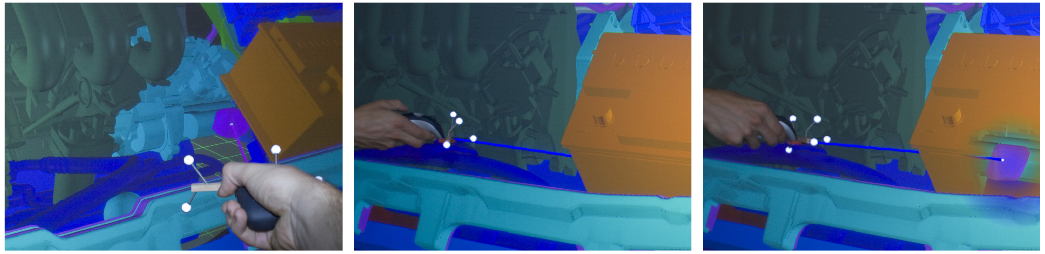
\includegraphics[width=12cm]{img/show_through_related.pdf}
	\end{center}
	\caption{Im linken Bild ist die freie Sicht auf die ausgewählte Geometrie möglich. Diese ist in der mittleren Darstellung verdeckt. In der rechten Abbildung schafft der durch \emph{Show-Through} nach Argelaguet et al. erzeugte Sichtkanal freien Blick auf die verdeckte Geometrie. Diese Abbildung entstammt vollständig einer Veröffentlichung von Argelaguet et al. \cite{argelaguet:2010}} 
	\label{fig:show_through_related}
\end{figure}

Wie in Abbildung \ref{fig:show_through_related} veranschaulicht wird nutzen Argelaguet et al. den von ihnen als \emph{Show-Through} bezeichneten Ansatz zur Freilegung verdeckter virtueller Objekte \cite{argelaguet:2010}. Bei perspektivischem Rendering kann der Blick auf verdeckte Objekte in manchen Betrachtungswinkeln auf der Projektionsfläche sichtbar sein. Die Auswahl dieser Geometrie schafft bei durch \emph{Show-Through} nach Argelaguet et al. einen Sichtkanal auf diese Inhalte für jeden Betrachtungswinkel. Im Kontext dieser Arbeit soll durch Anwendung der Technik die von der Hand des Nutzers durchstoßene Geometrie oberhalb der Projektionsfläche entfernt werden.

\begin{figure}
	\begin{center}
		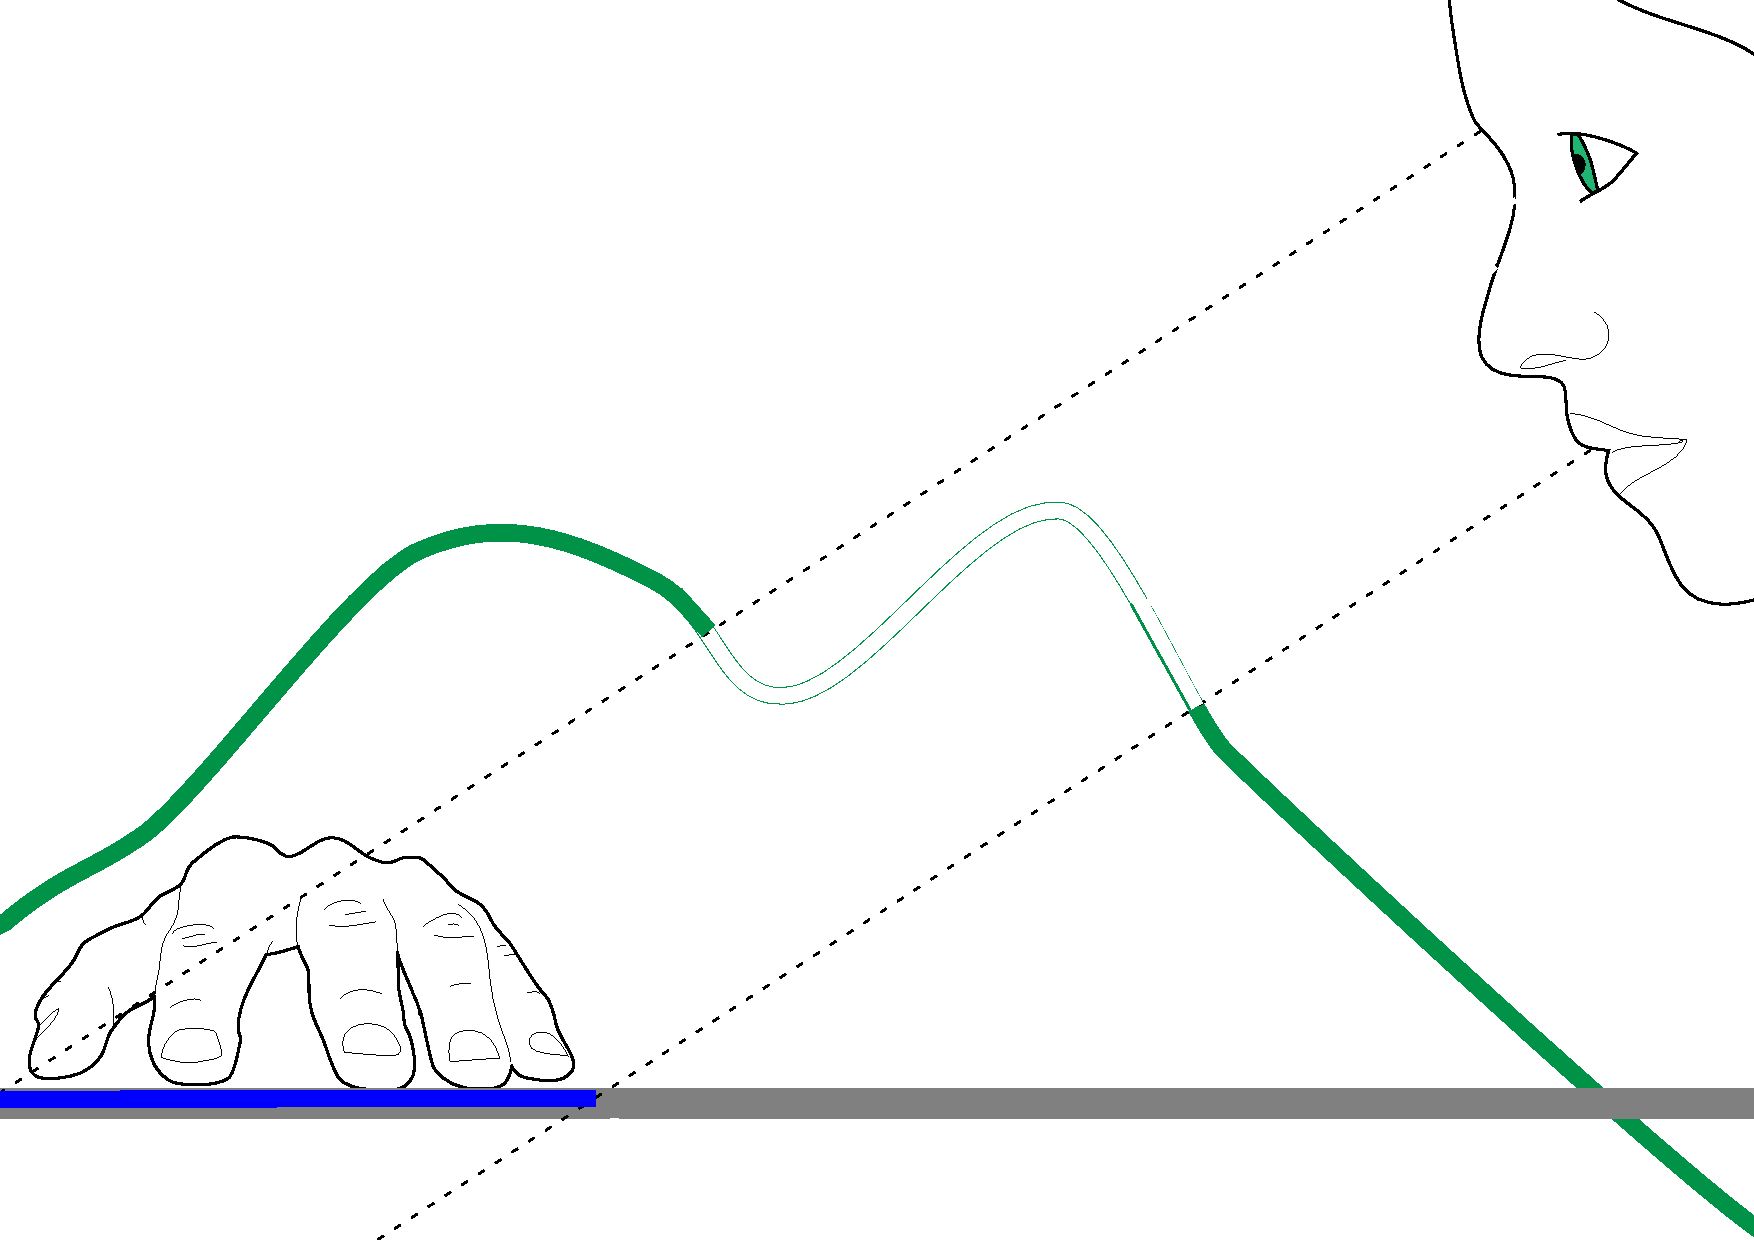
\includegraphics[width=12cm]{img/see_through_1.pdf}
	\end{center}
	\caption{Visualisierung des \emph{See-Through} Konzepts. Die blaue Fläche referenziert das Areal des fingerumschließenden Kreises}
	\label{fig:see_through_1}
\end{figure} 

Wird die Tischoberfläche berührt, so werden negativ parallaxe Modellbereiche zwischen der Eingabeposition und dem Kopf des Nutzers in einem bestimmten Durchmesser ausgeschnitten. Dies erzeugt einen zylinderförmigen Blicktunnel, welcher dem Nutzer freie Sicht bis zu seiner Hand auf der Tischebene bietet. Der Durchmesser des Ausschnittzylinders wird hierbei durch den fingerumschließenden Kreis bestimmt. Abbildung \ref{fig:see_through_1} illustriert die Anwendung der Technik.
\\\\
In einem Mehrbenutzerszenario wird für jeden Nutzer eine eigene Projektion der virtuellen Szene auf dem Bildschirmtisch erstellt. Dies beeinflusst auch die Perspektive auf von Händen verdeckte, negativ parallaxe, Bereiche der Darstellung. Wird für alle um den Tisch versammelten Personen der gleiche Ausschnittzylinder verwendet, kann ausschließlich für einen der Nutzer eine konfliktfreie Wahrnehmung sichergestellt werden.
\\\\
Um Wahrnehmungskonflikte für alle Anwender vermeiden zu können, muss die Orientierung des Ausschnittzylinders nutzerspezifisch angepasst werden. Infolgedessen wird eine eigene Repräsentation des Zylinders für jeden Nutzer bestimmt und auf die jeweilige Projektion angewandt.


\section{Implementierung}
\label{sec:implementierung_freischneiden}

Die Anwendung der \emph{See-Through} Technik kann leicht beim Rendern der Geometriefragmente vorgenommen werden. Hierzu werden alle Eingabepositionen der Hände auf der Tischfläche, sowie der Radius des fingerumschließenden Kreises, in den Fragmentshader der Applikation gegeben. Die Position der Kamera entspricht der Kopfposition des Nutzers und kann somit zur nutzerspezifischen Berechnung der Orientierung des Ausschnittzylinders genutzt werden. Zuletzt werden alle Fragmente, welche innerhalb des Blicktunnels liegen, verworfen.


\section{Vorteile und Limitierungen}
\label{sec:vorteile_und_limitierungen_freischneiden}

Durch die Anwendung der \emph{See-Through} Technik können blickabhängig, von der Hand verdeckte, negativ parallaxe Modellausschnitte bei der Projektion der virtuellen Szene ausgeschlossen werden. Hierdurch bleibt die geometrische Relation zwischen realen und virtuellen Inhalte erhalten. Dies führt zu einer wahrnehmungsunterstützenden Visualisierung, welche maßgeblich zur Benutzbarkeit der Toucheingaben beiträgt.
\\\\
Die \emph{See-Through} Technik beeinflusst lediglich die Darstellung der virtuellen Szene. Eine Manipulation der Geometrie, oder des Blickpunktes, wird nicht vorgenommen. Dadurch kann mit der Szene in jeder geometrischen Lage interagiert werden.
\\\\
Der Zylinder als Ausschnittgeometrie hat sich in der prototypischen Anwendung als gute Approximation des Nutzerarmes erwiesen. Es ist damit möglich den Großteil verdeckter, negativ parallaxer Modellausschnitte, von der Darstellung auszuschließen.
\\\\
Die Ausschnittgeometrie umschließt jedoch ein Volumen, welches nicht exakt die Gliedmaßen des Nutzers repräsentiert. Infolgedessen können Bereiche der Visualisierung beschnitten werden, welche nicht vom Nutzer verdeckt werden und daher noch sichtbar sein sollten. Des Weiteren entspricht die Form und Orientierung der Ausschnittgeometrie nicht der komplexen Form des Arms eines Nutzers. Bei bestimmten Eingaben können somit nicht alle durch Negativparallaxe hervorgerufenen Wahrnehmungskonflikte vermieden werden.
\\\\
Die \emph{See-Through} Technik wird durch das Berühren der Bildschirmoberfläche initiiert. Aus diesem Grund kann das Hineingreifen in Inhalte oberhalb dieser Ebene, ohne Interaktion mit der Tischfläche, nicht verhindert werden.